\section{Tricks}

In this section are described random tricks used to speed up rendition. They range from simple precomputed cos/sin tables to what I consider one of the most beautiful hack in the engine: Linear Feedback Shit Register.




\subsection{Cos/Sin table lookup}
\cw{cos} and \cw{sin} are expensive methods involving floating point calculation. They are extensively used at runtime. To speed things up, at startup, the engine generates and cache them in a lookup array (one value per angle). So save RAM, it exploits a math property ($cos(X) = sin(X + 90)$) to avoid 360 \cw{cos} method calls and 240 bytes of RAM by reusing the cos table as follow:\\
\par

\begin{minipage}{\textwidth}
\lstinputlisting[language=C]{code/sin_cos_table.c}
\end{minipage}


\begin{figure}[H]
 \centering
  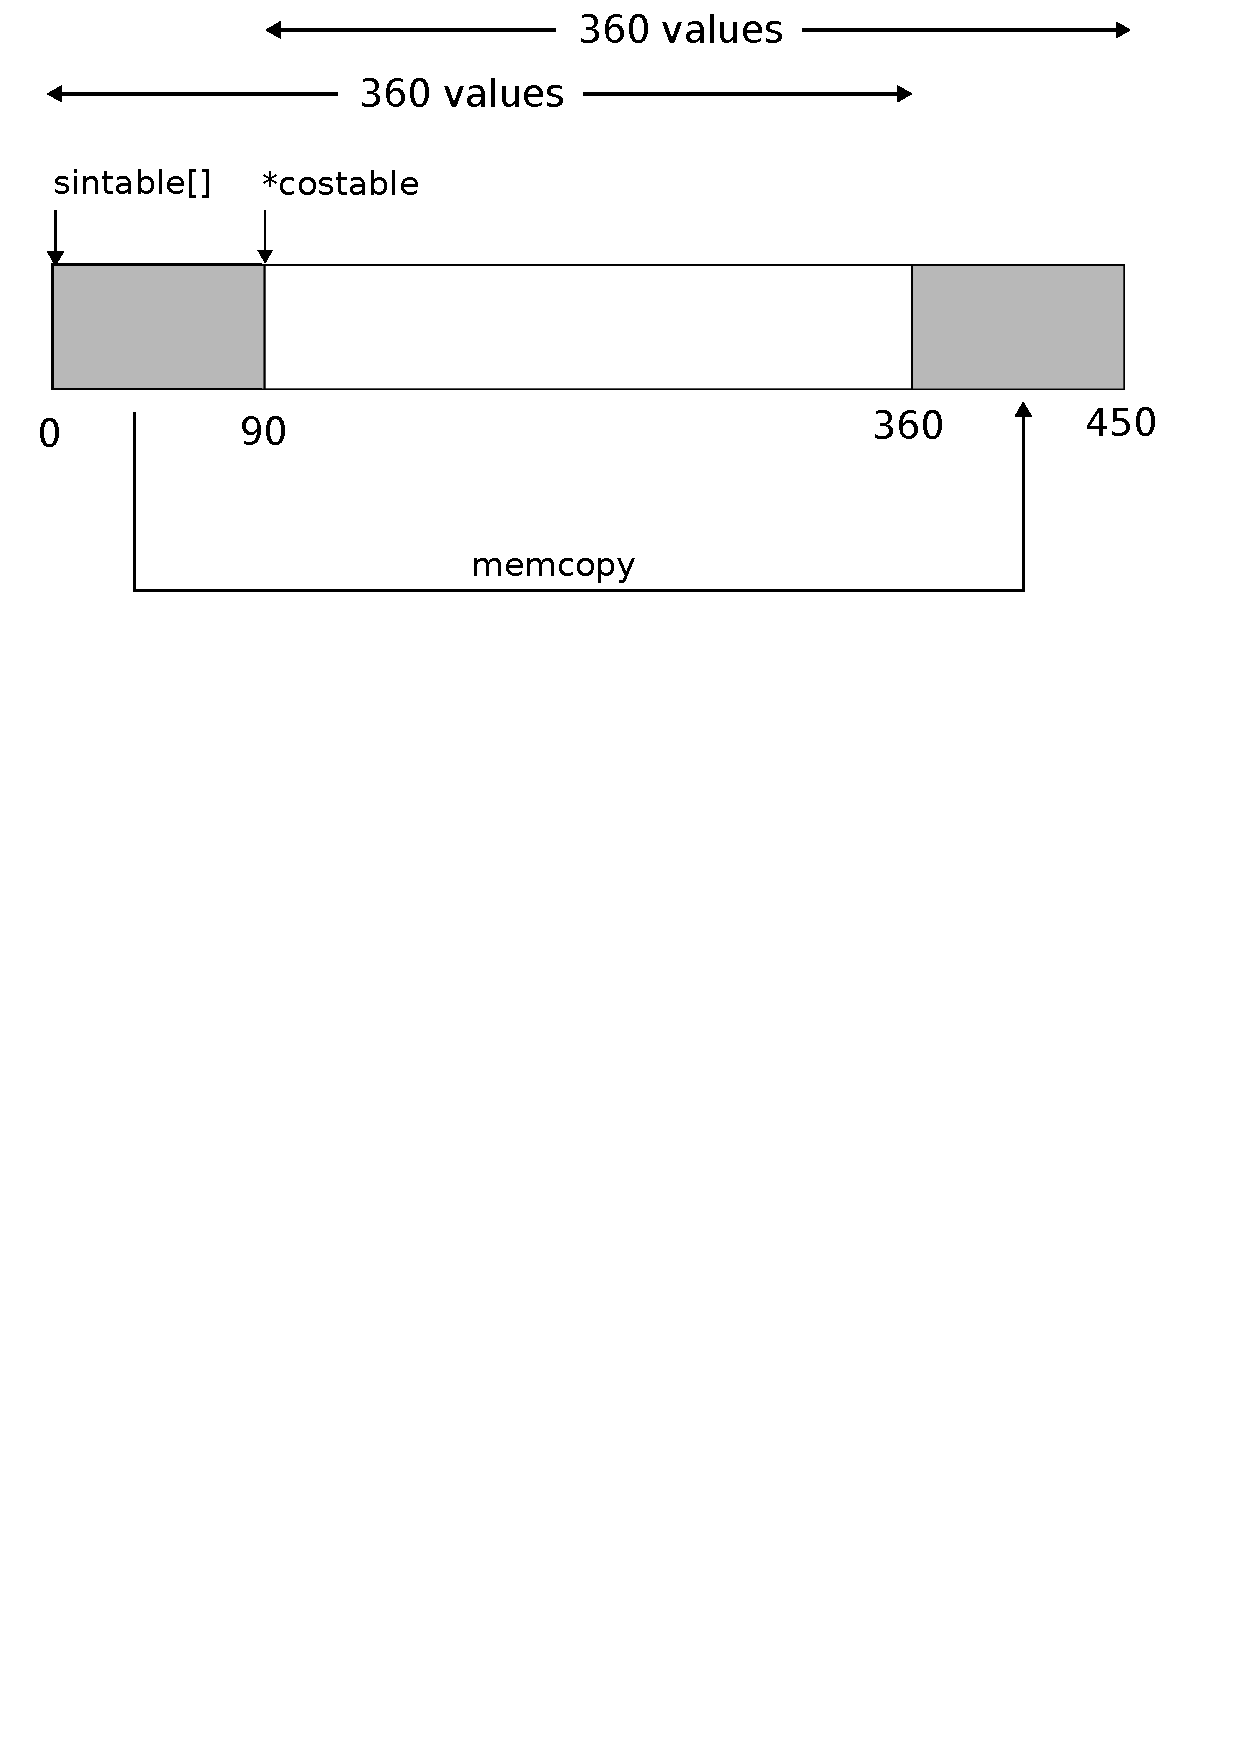
\includegraphics[width=\textwidth]{imgs/drawings/cos_sin_table.pdf}
 \caption{Finalez frame} 
\end{figure}








\subsection{FizzleFade}
While most screen transition are done with a black fade effect (by shifting the palette), there are two instances
when the screen transition via fizzling:
\begin{itemize}
	\item When dying
	\item When killing a boss
\end{itemize}




\begin{minipage}{\textwidth}
\centering
  \scaledimage{.9}{fizzlefade/dying/screenshot_16.png}\\
  \vspace*{0.5cm}
  \scaledimage{.9}{fizzlefade/dying/screenshot_19.png}\\
\end{minipage}

\begin{minipage}{\textwidth}
\centering
  \scaledimage{.9}{fizzlefade/dying/screenshot_52.png} \\
  \vspace*{0.5cm}
  \scaledimage{.9}{fizzlefade/dying/screenshot_86.png} \\
\end{minipage}


\begin{minipage}{\textwidth}
\centering
  \scaledimage{.9}{fizzlefade/boss/screenshot_60.png} \\
  \vspace*{0.5cm}
  \scaledimage{.9}{fizzlefade/boss/screenshot_66.png}  \\
\end{minipage}

\begin{minipage}{\textwidth}
\centering
  \scaledimage{.9}{fizzlefade/boss/screenshot_102.png}\\
\vspace*{0.5cm}
  \scaledimage{.9}{fizzlefade/boss/screenshot_130.png}\\
\end{minipage}

A naive approach would have been to reuse the pseudo random generator \cw{US\_RndT} and keep track of which pixels had been fizzled. But that would make the fade non-deterministic with regard to duration and that would also be a waste of CPU cycles since a same pixel coordinate (X,Y) could come up several times. There is a much faster and elegant way to do it. The code responsible for this effect can be found in id\_vh.cpp, function FizzleFade. At first it is not obvious to understand how it works.\\
\par
\begin{minipage}{\textwidth}
\lstinputlisting[language=C]{code/fizzlefade.c}
\end{minipage}
\par
Which can be read as:\\
\begin{itemize}
\item Initialize \cw{rndval} to 1.
\item Break it down in 8 + 7 bits: Use 8 bits generate an X coordinate and 7 bits for a Y coordinate.
\item Subject \cw{rndval} to a soup of XORing.
\item When \cw{rndval} value is somehow back to 1: Stop.
\end{itemize}        
It looks like magic at first. How is \cw{rndval} supposed to return to value 1?! That technique is called Linear Feedback Shit Register. To make it work, one needs a register which will be right shifted each iteration. Since it is right shifted, the right bit disappears and a new one to the left is needed. To generate this new bit, the register use "taps" which are bit offset used to XOR together values and generate the new bit value. A Fibonnaci representation shows a simple LFSR with one tap.\\
\par

\begin{figure}[H]
 \centering
  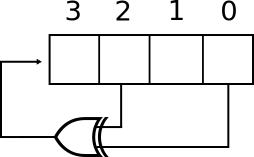
\includegraphics[width=.4\textwidth]{imgs/drawings/4bits_lfsr.pdf}
 \caption{Finalez frame} 
\end{figure}
This register is able to generate 7 values before it cycle back to it original state. The following listing shows all of them.
\par
\begin{minipage}{\textwidth}
\lstinputlisting[language=C]{code/lfsr.txt}
\end{minipage}
\par
Since the VGA framebuffer needs at least 320x200 values, it uses a 17 bits LFSR with two taps.\\
\par
\begin{figure}[H] \centering 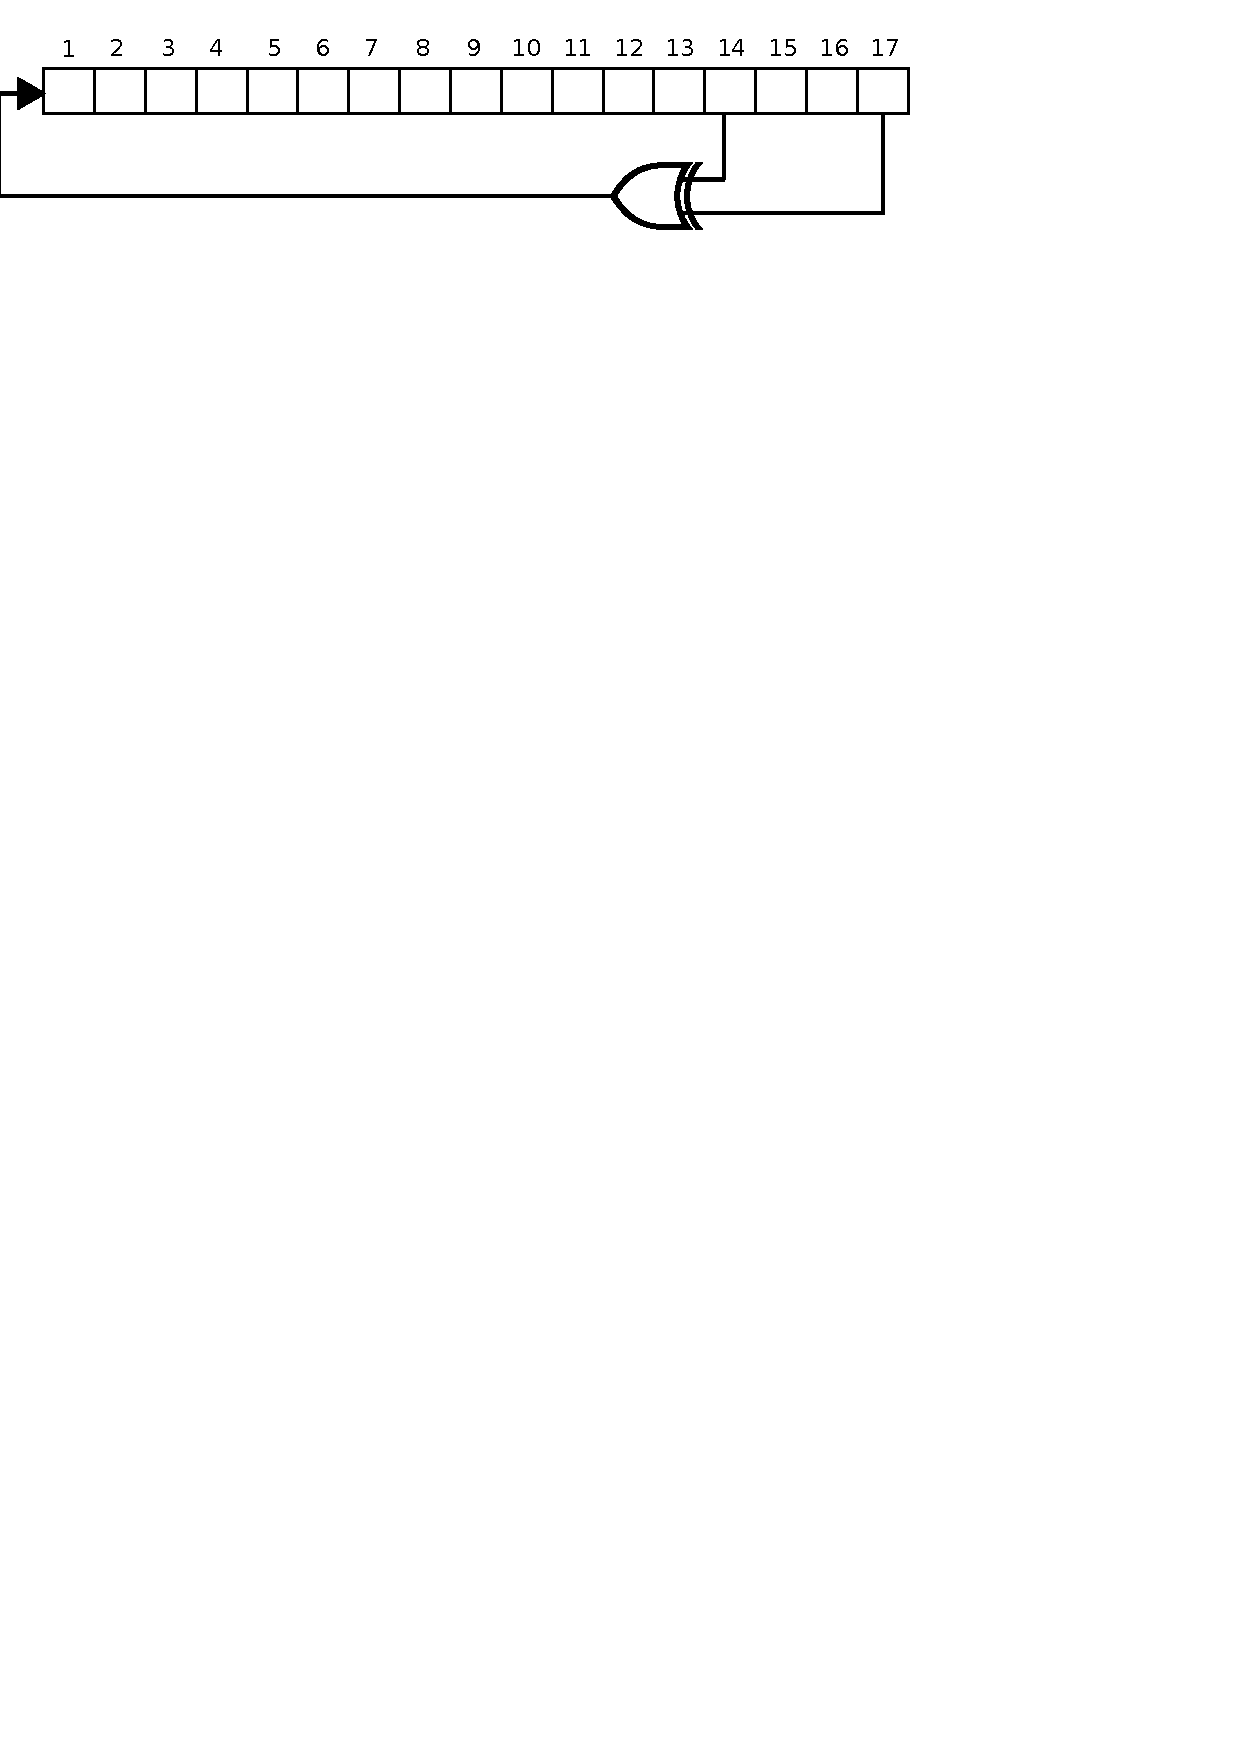
\includegraphics[width=\textwidth]{imgs/drawings/fizzlefade/fibonacci.pdf} \end{figure}
\par
The above diagram is slow to implement in software. There is an alternative way to represent a LFSR called "Galois" and this is the way Wolfenstein 3D implements its LFSR and writes 320x200=64000 exactly once.
\par
\begin{figure}[H] \centering 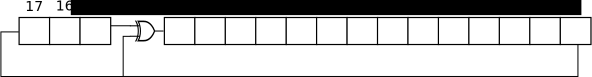
\includegraphics[width=\textwidth]{imgs/drawings/fizzlefade/galois.pdf} \end{figure}
      
\bu{Note :} Because the effect works by plotting pixels individually, this effect was very hard to replicate when developers tried to port the game to hardware accelerated GPU. As far as I know none of the port managed to replicate the fizzlefade.\\
\par
\bu{Note :} If you are curious about maximum-length taps, xilinx provides them from 3 to 168\footnote{Xilinx table can be found \href{http://www.xilinx.com/support/documentation/application\_notes/xapp052.pdf}{here}.}.










\subsection{Palette}
Even though it limit the graphic capabilities, the palette system can be turned into a strength. It is easy to fade the screen to white (when picking up an item), red (when taking damages) or back (for transition between 2D menus). It only takes 256*3 = 768 bytes and 768 out instructions to modify the full screen.
\begin{figure}[H]
  \centering
 \fullimage{palette_damage.png}
 \caption{The palette RGB colors altered when taking damage.} \label{fig:palette_damage}
\end{figure}
A fast path is provided (which ironically only works if the CPU is as slow at the VGA) to update the palette via one \cw{lobsb} instruction. Otherwise if not supported a loop of 768 \cw{outsb} is used.\\
\par
\begin{minipage}{\linewidth}
\lstinputlisting[language=C,morekeywords={asm,byte,far}]{code/vl_setpalette.c}
\end{minipage}








\section{Pseudo random generator}
\note{Elaborate}
\begin{minipage}{\textwidth}
\lstinputlisting[language={[x86masm]Assembler}, style=mystyle,basicstyle=\small]{code/rndtable.asm}
\end{minipage}

\begin{minipage}{\textwidth}
\lstinputlisting[language={[x86masm]Assembler}]{code/US_InitRndT.asm}
\end{minipage}


\begin{minipage}{\textwidth}
\lstinputlisting[ language={[x86masm]Assembler}]{code/US_RndT.asm}
\end{minipage}








